%%%%%%%%%%%%%%%%%%%%%%%%%%%%%%%%%%%%%%%%%%%%%%%%%%%%%%%%%%%%%%%%%%%%%%%%%%%%%%%%
\section{A first Workflow}

%%%%%%%%%%%%%%%%%%%%%%%%%%%%%%%%%%%%%%%%%%%%%%%%%%%%%%%%%%%%%%%%%%%%%%%%%%%%%%%%
\begin{frame}
    \frametitle{Outline}
    \begin{columns}[t]
        \begin{column}{.5\textwidth}
            \tableofcontents[sections={1-9},currentsection]
        \end{column}
        \begin{column}{.5\textwidth}
            \tableofcontents[sections={10-18},currentsection]
        \end{column}
    \end{columns}
\end{frame}

%%%%%%%%%%%%%%%%%%%%%%%%%%%%%%%%%%%%%%%%%%%%%%%%%%%%%%%%%%%%%%%%%%%%%%%%%%%%%%%%
\begin{frame}
  \frametitle{What is this about?}
   \question[Questions]{How do I write a simple workflow?}
   \docs[Objectives]{\begin{enumerate}
                      \item Understand the components of a Snakefile: rules, inputs, outputs, and actions.
                      \item Write a simple Snakefile.
                      \item Run Snakemake from the shell.
                     \end{enumerate}}
\end{frame}

%%%%%%%%%%%%%%%%%%%%%%%%%%%%%%%%%%%%%%%%%%%%%%%%%%%%%%%%%%%%%%%%%%%%%%%%%%%%%%%
\begin{frame}[fragile]
  \frametitle{Before we begin \ldots}
  \begin{exampleblock}{Working with closure Files}
    To ease the excercises and save typing time, all excercises are supplied as cloze texts.\linebreak
    \texttt{Snakemake} relies on a file called \texttt{Snakefile} to be present. You can either rename your cloze texts like
    \begin{lstlisting}[language=Bash, style=Shell]
$ cp <number>_Snakefile Snakefile
    \end{lstlisting}
    or specify the workflow file on the commandline with an additional flag:
    \begin{lstlisting}[language=Bash, style=Shell]
$ snakemake <other arguments> \
> --snakefile <number>_Snakefile
    \end{lstlisting}
    Also note: \altverb{\\} may denote a linebreak in \texttt{Bash} and \altverb{>} its continuation. Omit these and you have a one-liner. It merely serves to fit text on screen, here.
  \end{exampleblock}
\end{frame}


%%%%%%%%%%%%%%%%%%%%%%%%%%%%%%%%%%%%%%%%%%%%%%%%%%%%%%%%%%%%%%%%%%%%%%%%%%%%%%%%
\subsection{A first Step or ``Rule''}

%%%%%%%%%%%%%%%%%%%%%%%%%%%%%%%%%%%%%%%%%%%%%%%%%%%%%%%%%%%%%%%%%%%%%%%%%%%%%%%%
\begin{frame}[fragile]
  \frametitle{Layout of a Workflow Development Directory} 
  \task{We are going to work in the \altverb{zipf\_analysis}-folder. Please \altverb{cd} there.}
  \pause
  The idea is to have a neat overview:
  \begin{columns}
    \begin{column}{0.5\textwidth}
      
  \begin{minipage}[t]{0.5\textwidth}
    \setstretch{0.1}
            {\tiny \DTsetlength{0.2em}{1em}{0.2em}{0.4pt}{.6pt}
\dirtree{%
.1 {\textit{workflow\ folder}}.
.2 {scripts}.
.3 {some\ scriptfile.py}.
.3 {some\ scriptfile.sh}.
.3 {some\ scriptfile.R}.
.2 {Snakefile}.
.2 {and more \ldots}.
}}
    \end{minipage}
    \end{column}
    \begin{column}{0.5\textwidth}
      \hint{Our long term goal:\newline Have a orderly overview and seperation of data and code.}
    \end{column}
  \end{columns}
\end{frame}

%%%%%%%%%%%%%%%%%%%%%%%%%%%%%%%%%%%%%%%%%%%%%%%%%%%%%%%%%%%%%%%%%%%%%%%%%%%%%%%%
\begin{frame}[fragile]
  \frametitle{Our first \texttt{Snakefile}!}
  \begin{onlyenv}<1| handout:0>
    Our first ``\altverb{rule}''. 
    \begin{lstlisting}[language=Python,style=Python]
rule bwa_map:
    input:
        "data/genome.fa",
        "data/samples/A.fastq"
    output:
        "mapped_reads/A.bam"
    shell:
        "bwa mem data/genome.fa"
        " data/samples/A.fastq"
        " | samtools view -Sb - >"
        " mapped_reads/A.bam"
    \end{lstlisting}
    \docs{This code is build file, which for \texttt{Snakemake} is called a \texttt{Snakefile} -- a file executed by \texttt{Snakemake}.}
    \end{onlyenv}
  \begin{onlyenv}<2| handout:0>
   We are going to ``map'' our reads onto the genome.
   \begin{lstlisting}[language=Python,style=Python]
rule @bwa_map@:
    input:
        "data/genome.fa",
        "data/samples/A.fastq"
    output:
        "mapped_reads/A.bam"
    shell:
        "bwa mem data/genome.fa"
        " data/samples/A.fastq"
        " | samtools view -Sb - >"
        " mapped_reads/A.bam"
    \end{lstlisting}
    For this we are using \lhref{https://github.com/lh3/bwa}{\altverb{bwa}}, specifically \altverb{bwa mem}. We call our rule accordingly \altverb{bwa_map}.
  \end{onlyenv}
  \begin{onlyenv}<3| handout:0>
   \altverb{input}, \altverb{output} and \altverb{shell} are called ``directives'':
   \begin{lstlisting}[language=Python,style=Python]
rule bwa_map:
    @input@:
        "data/genome.fa",
        "data/samples/A.fastq"
    @output@:
        "mapped_reads/A.bam"
    @shell@:
        "bwa mem data/genome.fa"
        " data/samples/A.fastq"
        " | samtools view -Sb - >"
        " mapped_reads/A.bam"
    \end{lstlisting}
    The \altverb{input} and \altverb{output} directives are followed by lists of files that are expected to be used or created by the rule. In the simplest case, these are just explicit Python strings.
  \end{onlyenv}
  \begin{onlyenv}<4| handout:0>
   The \altverb{shell} may be one line or contain line breaks:
  \begin{lstlisting}[language=Python,style=Python]
rule bwa_map:
    input:
        "data/genome.fa",
        "data/samples/A.fastq"
    output:
        "mapped_reads/A.bam"
    shell:
        @"bwa mem data/genome.fa"
        " data/samples/A.fastq"
        " | samtools view -Sb - >"
        " mapped_reads/A.bam"@
    \end{lstlisting}
    \bcattention Python will concatenate those Strings! Be sure to include spaces to make up a valid command in Bash.
  \end{onlyenv}
  \begin{onlyenv}<5| handout:1>
   Be sure to have copied everything to your \texttt{Snakefile} and save it.
   \begin{lstlisting}[language=Python,style=Python]
rule bwa_map:
    input:
        "data/genome.fa",
        "data/samples/A.fastq"
    output:
        "mapped_reads/A.bam"
    shell:
        "bwa mem data/genome.fa"
        " data/samples/A.fastq"
        " | samtools view -Sb - >"
        " mapped_reads/A.bam"
    \end{lstlisting}
  \end{onlyenv}
\end{frame}

%%%%%%%%%%%%%%%%%%%%%%%%%%%%%%%%%%%%%%%%%%%%%%%%%%%%%%%%%%%%%%%%%%%%%%%%%%%%%%%%
\begin{frame}
  \frametitle{\texttt{Snakefile}s are Python Files}
  \begin{block}{Some Background}
     \begin{enumerate}
       \item Like Python, you can use either tabs or spaces for indentation — don’t mix!
       \item Together, the target, dependencies, and actions form a rule. A rule is a recipe for how to make things.
  \end{enumerate}
  \end{block}
\end{frame}


%%%%%%%%%%%%%%%%%%%%%%%%%%%%%%%%%%%%%%%%%%%%%%%%%%%%%%%%%%%%%%%%%%%%%%%%%%%%%%%%
\begin{frame}[fragile]
  \frametitle{Finally - Running \texttt{Snakemake}!}
  Now, we can run \texttt{Snakemake}:
  \begin{lstlisting}[language=Bash, style=Shell]
$ snakemake --cores=1
  \end{lstlisting}
  \hint[Note:]{The \altverb{--cores=1} is necessary, because we are executing ``locally'' and \texttt{Snakemake} would like to know how much of the resources we may use (you can try without, though, to see what happens).}
  You should see the expected output (\altverb[Bash]{ls}) and lines which reads:
  \begin{lstlisting}[style=Plain, basicstyle=\footnotesize]
1 of 1 steps (100%) done
Complete log: .snakemake/log/2022-09-17T145657.968906.snakemake.log
  \end{lstlisting}
\end{frame}

%%%%%%%%%%%%%%%%%%%%%%%%%%%%%%%%%%%%%%%%%%%%%%%%%%%%%%%%%%%%%%%%%%%%%%%%%%%%%%%%
\begin{frame}[fragile]
  \frametitle{Re-Running Workflows}
  Try to run \texttt{Snakemake} again:
  \begin{lstlisting}[language=Bash, style=Shell]
$ snakemake --cores=1
  \end{lstlisting}
  \pause
  Oops:
  \begin{lstlisting}[style=Plain, basicstyle=\footnotesize]
Nothing to be done (all requested files are present and up to date).
  \end{lstlisting}
  \pause
  Now, do:
  \begin{lstlisting}[language=Bash, style=Shell]
$ touch ../books/isles.txt
$ ls -l ../* # will proove: the input is more 
          # recent the the output
  \end{lstlisting}
  And run \texttt{Snakemake} once more.
  \question{What happens? Why?}
\end{frame}

%%%%%%%%%%%%%%%%%%%%%%%%%%%%%%%%%%%%%%%%%%%%%%%%%%%%%%%%%%%%%%%%%%%%%%%%%%%%%%%%
\begin{frame}
  \frametitle{When do Rules get executed? - The Solution}
  When it is asked to build a target, \texttt{Snakemake} checks the “last modification time” of both the \emph{target} and its \emph{dependencies}.
  If either
  \begin{itemize}
   \item any dependency has been updated
   \item or a job failed to produce a target (completely)
  \end{itemize}
  upon re-run \texttt{Snakemake} will only rebuild the files that, either directly or indirectly, depend on the file that changed. This is called an \emph{incremental build}.
  \pause
  \docs{By explicitly recording the inputs to and outputs from steps in our analysis and the dependencies between files, Snakefiles act as a type of documentation, reducing the number of things we have to remember.}
\end{frame}

%%%%%%%%%%%%%%%%%%%%%%%%%%%%%%%%%%%%%%%%%%%%%%%%%%%%%%%%%%%%%%%%%%%%%%%%%%%%%%%%
\begin{frame}[fragile]
  \frametitle{\HandsOn{Proceeding naively}}
  Let’s add another rule to the end of \texttt{Snakefile}. Take the template \texttt{02\_Snakemake}. Note that rules cannot have the same name, so we’ll call this one \altverb{count_words_abyss}.
\end{frame}

%%%%%%%%%%%%%%%%%%%%%%%%%%%%%%%%%%%%%%%%%%%%%%%%%%%%%%%%%%%%%%%%%%%%%%%%%%%%%%%%
\begin{frame}[fragile]
   \frametitle{Proceeding naively II}
   This should give us:
  \begin{lstlisting}[language=Python,style=Python]
rule count_words_abyss:
    input:    '../books/abyss.txt'
    output:   'abyss.dat'
    shell:    'python scripts/wordcount.py' 
               ' -i ../books/abyss.txt -o abyss.dat'
  \end{lstlisting}
  \task{Run \texttt{Snakemake} - what happens?}
\end{frame}

%%%%%%%%%%%%%%%%%%%%%%%%%%%%%%%%%%%%%%%%%%%%%%%%%%%%%%%%%%%%%%%%%%%%%%%%%%%%%%%%
\begin{frame}[fragile]
  \frametitle{Rules need targets!}
  Nothing happens because \texttt{Snakemake} attempts to build the first target it finds in the Snakefile, the default target, which is \altverb{isles.dat} which is already up-to-date. We need to explicitly tell \texttt{Snakemake} we want to build \altverb{abyss.dat}:
  \begin{lstlisting}[language=Bash, style=Shell]
$ snakemake --cores=1 abyss.dat
  \end{lstlisting}
\end{frame}

%%%%%%%%%%%%%%%%%%%%%%%%%%%%%%%%%%%%%%%%%%%%%%%%%%%%%%%%%%%%%%%%%%%%%%%%%%%%%%%%
\begin{frame}[fragile]
  \frametitle{``Up to Date'' Versus ``Nothing to be Done''}
  If we ask \texttt{Snakemake} to build a file that already exists and is up to date, then \texttt{Snakemake} informs us that:
  \begin{lstlisting}[style=Plain]
Nothing to be done
  \end{lstlisting}
  \pause
  If we ask \texttt{Snakemake} to build a file that exists but for which there is no rule in our Snakefile, then we get a message like:
  \begin{lstlisting}[language=Bash, style=Shell, basicstyle=\footnotesize]
$ snakemake --cores=1 scripts/wordcount.py
# skipping some output
MissingRuleException:
No rule to produce wordcount.py (if you use input functions make sure
that they don't raise unexpected exceptions).
  \end{lstlisting}
  \hint{When we see this error, double-check that you have a rule to produce that file, and also that the filename has been specified correctly. Even a small difference in a filename will result in a \texttt{MissingRuleException}.}
\end{frame}

%%%%%%%%%%%%%%%%%%%%%%%%%%%%%%%%%%%%%%%%%%%%%%%%%%%%%%%%%%%%%%%%%%%%%%%%%%%%%%%%
\begin{frame}[fragile]
  \frametitle{Rules without Outputs?!}
  We may want to remove all our data files so we can explicitly recreate them all. We can introduce a new target, and associated rule, to do this. We will call it clean, as this is a common name for rules that delete auto-generated files, like our \altverb{.dat} files:
  \begin{lstlisting}[language=Python,style=Python]
rule clean:
    shell: 'rm -f *.dat'
  \end{lstlisting}
  There are no in- or outputs! When we invoke the rule, 
  \begin{lstlisting}[language=Bash, style=Shell]
$ snakemake --cores=1 clean
  \end{lstlisting}
  our  \altverb{.dat} files are deleted.
\end{frame}

%%%%%%%%%%%%%%%%%%%%%%%%%%%%%%%%%%%%%%%%%%%%%%%%%%%%%%%%%%%%%%%%%%%%%%%%%%%%%%%%
\begin{frame}[fragile]
  \frametitle{Rules without Outputs?! - II }
  We can add a similar command to create all the data files. We can put this \textbf{at the top} of our Snakefile so that it is the default target, which is executed by default if no target is given to the snakemake command:
  \begin{lstlisting}[language=Python,style=Python]
rule dats:
    input:
        'isles.dat'@,@
        'abyss.dat'
  \end{lstlisting}
  This rule is also an example of a rule that has no actions. It is used purely to trigger the build of its dependencies, if needed.

  If we run,
  \begin{lstlisting}[language=Bash, style=Shell] 
$ snakemake --cores=1 dats
  \end{lstlisting}
  \texttt{Snakemake} creates these missing files.
\end{frame}

%%%%%%%%%%%%%%%%%%%%%%%%%%%%%%%%%%%%%%%%%%%%%%%%%%%%%%%%%%%%%%%%%%%%%%%%%%%%%%%%
\begin{frame}[fragile]
  \frametitle{Dependencies form a DAG!}
  \begin{exampleblock}{Dependencies}
    The order of rebuilding dependencies is arbitrary. You should not assume that they will be built in the order in which they are listed.
    Dependencies must form a directed acyclic graph (DAG). A target cannot depend on a dependency which itself, or one of its dependencies, depends on that target.
  \end{exampleblock}
  If we run dats again, then snakemake will see that the dependencies (\altverb{isles.dat} and \altverb{abyss.dat}) are already up to date. Given the target dats has no actions, there is nothing to be done:
  \begin{lstlisting}[language=Bash, style=Shell] 
$ snakemake --cores=1 dats
# ...
Nothing to be done
  \end{lstlisting}
\end{frame}

%%%%%%%%%%%%%%%%%%%%%%%%%%%%%%%%%%%%%%%%%%%%%%%%%%%%%%%%%%%%%%%%%%%%%%%%%%%%%%%%
\begin{frame}[fragile]
  \frametitle{What do we have - UP TO NOW?}
  \begin{columns}
   \begin{column}{0.8\textwidth}
     Our ``Workflow'' so far:
     \begin{lstlisting}[language=Python,style=Python, basicstyle=\tiny]
rule dats:
     input:
         'isles.dat',
         'abyss.dat'

# delete everything so we can re-run things
rule clean:
    shell: 'rm -f *.dat'

# count words in one of our "books"
rule count_words:
    input:    'books/isles.txt'
    output:   'isles.dat'
    shell:    'python scripts/wordcount.py'
              ' -i books/isles.txt -o isles.dat'

rule count_words_abyss:
    input:    'books/abyss.txt'
    output:   'abyss.dat'
    shell:    'python scripts/wordcount.py' 
              ' -i books/abyss.txt -o abyss.dat'     
     \end{lstlisting}

   \end{column}
   
   \begin{column}{0.2\textwidth}
     The DAG can be graphed like this:
     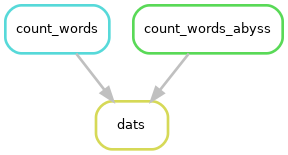
\includegraphics[width=\textwidth]{workflows/mini_dag.png}
     2 producers, a single target rule.
   \end{column}
  \end{columns}
\end{frame}

%%%%%%%%%%%%%%%%%%%%%%%%%%%%%%%%%%%%%%%%%%%%%%%%%%%%%%%%%%%%%%%%%%%%%%%%%%%%%%%%
\begin{frame}[fragile]
  \frametitle{\HandsOn{Add some Stuff!}}
  \begin{enumerate}
   \item Write a new rule for \altverb{last.dat}, created from \altverb{../books/last.txt}.
   \item Write a new rule for \altverb{results.txt}, which creates the summary table. The rule needs to:
        \begin{itemize}
         \item Depend upon each of the three .dat files.
         \item Invoke the action \altverb{python scripts/zipf_test.py abyss.dat isles.dat last.dat > results.txt}\,.
        \end{itemize}
   \item Update the \altverb{dats} rule with this target. Do we still need the \altverb{*dat} files as target?
   \item Put this rule at the top of the Snakefile so that it is the default target.
   \item Update clean so that it removes \altverb{results.txt}.
  \end{enumerate}
  \hint{Please refer to cloze text \texttt{03\_Snakefile}.}
\end{frame}


%%%%%%%%%%%%%%%%%%%%%%%%%%%%%%%%%%%%%%%%%%%%%%%%%%%%%%%%%%%%%%%%%%%%%%%%%%%%%%%%
\begin{frame}[fragile]
Our little exercise should produce this Workflow:
  \begin{columns}
    \begin{column}{0.5\textwidth}
      \begin{lstlisting}[language=Python,style=Python, basicstyle=\tiny]
rule dats:
     input:
         'results.txt'

# delete everything so we can re-run things
rule clean:
    shell: 'rm -f *.dat results.txt'

# count words in one of our "books"
rule count_words:
    input:    '../books/isles.txt'
    output:   'isles.dat'
    shell:    'python scripts/wordcount.py'
              ' -i ../books/isles.txt'
              ' -o isles.dat'

rule count_words_abyss:
    input:    '../books/abyss.txt'
    output:   'abyss.dat'
    shell:    'python scripts/wordcount.py' 
              ' -i ../books/abyss.txt' 
              ' -o abyss.dat'
      \end{lstlisting}
    \end{column}
    \begin{column}{0.5\textwidth}
      \begin{lstlisting}[language=Python,style=Python, basicstyle=\tiny]
#continued ...
rule count_words_last:
    input:    '../books/last.txt'
    output:   'last.dat'
    shell:    'python scripts/wordcount.py'
              ' -i ../books/last.txt'
              ' -o last.dat'
              
# generate summary table
rule zipf_test:
    input:  'abyss.dat', 'last.dat', 
            'isles.dat'
    output: 'results.txt'
    shell:  'python scripts/zipf_test.py' 
            ' abyss.dat isles.dat last.dat'
            ' > results.txt'
      \end{lstlisting}
    \end{column}
  \end{columns}
\end{frame}


  

